\section{Supporting Figures}

\begin{figure}[H]
\centering
  \includegraphics[width=\textwidth]{sgeFigure_S1}
\caption{The conclusion in Fig. 1 is not dependent on the average
number of epistatic interaction partners per gene. (A) The
distribution of average number of epistatic interaction partners per
gene. For each gene with epistasis, its average number of epistatic
interaction partners was calculated among all mutant alleles of this
gene. (B-D) A similar conclusion to that of Fig. 1 can be obtained
when we only use genes with fewer than 500 (B), 500-2,000 (C), and
more than 2,000 (D) average epistatic interaction partners. The same
methods in Fig. 1 were used here to generate B-D.}
\label{fig:sgeS1}
\end{figure}

\begin{figure}[H]
\centering
  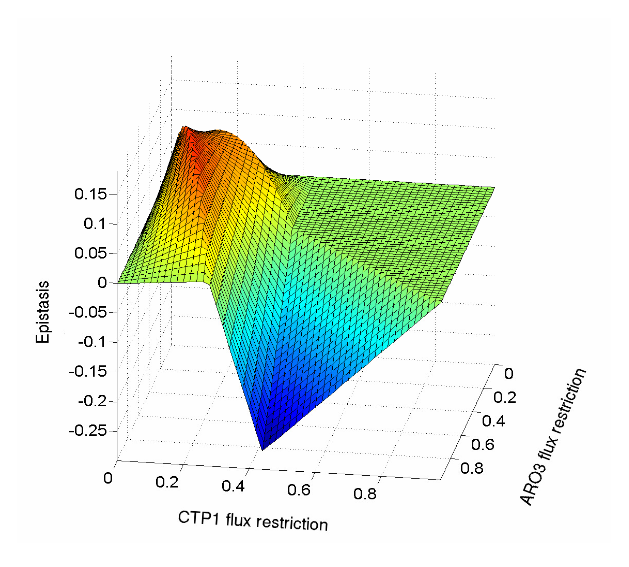
\includegraphics[width=\textwidth]{sgeFigure_S2}
\caption{A complex epistatic landscape exhibits a transition from
large positive to large negative epistasis values, along with a region
of zero epistasis. Epistasis is viewed as a function of the CTP1 and
ARO3 genes’ flux restriction. The color corresponds to the z-axis
(epistasis), with red being more positive, green being near zero, and
blue being more negative.}
\label{fig:sgeS2}
\end{figure}

\begin{figure}[H]
\centering
  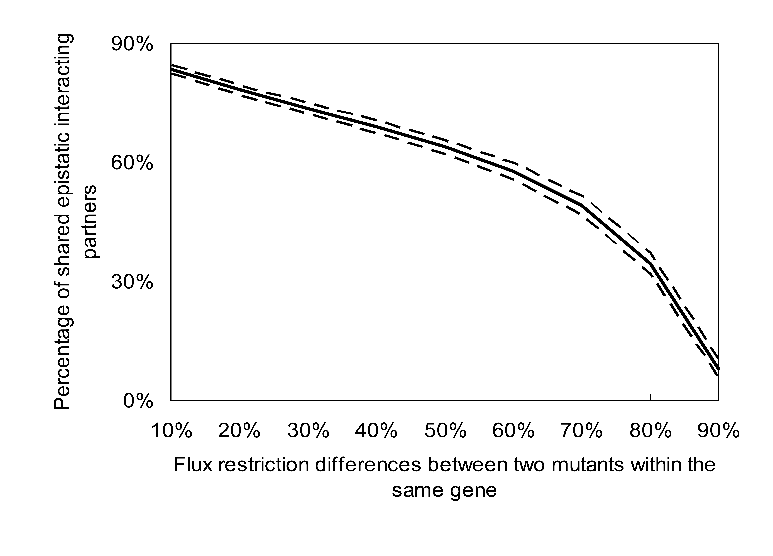
\includegraphics[width=\textwidth]{sgeFigure_S3}
\caption{Percentage of shared epistatic interacting partners based on
flux differences between two mutant alleles of the same gene. The
analysis procedure is the same as Fig. 1A, but instead of using the
S. cerevisiae model, here we repeated the analysis using the E. coli
model (38).}
\label{fig:sgeS3}
\end{figure}


\captionpage{figure}{%
The conclusion that epistatic relations between genes are
allele-specific is robust to various epistasis thresholds. Left 5
panels: The FBA simulation results for the distribution of the
percentage of shared epistatic interaction partners between two mutant
alleles within the same gene. Solid and broken lines represent mean
and 95\% confidence intervals, respectively. Right 5 panels: The
cumulative distribution for the percentage of shared epistatic
interaction partners between two mutant alleles within the same gene
based on real experimental data. Both experimental and simulated
results are robust under various epistasis thresholds.}
\label{fig:sgeS4}

\begin{figure}[H]
\centering
  \includegraphics[width=\textwidth]{sgeFigure_S4}
\end{figure}

\begin{figure}[H]
\centering
  \includegraphics[width=\textwidth]{sgeFigure_S5}
\caption{The conclusion in Fig. 3, for which mutant alleles with more
severe defects tend to have a higher percentage of negative epistasis
in eukaryotes than bacteria and archaea, is robust under various
epistasis and fitness difference thresholds. The same methods to
generate Fig. 2C for S. cerevisiae are used here for the other five
species.}
\label{fig:sgeS5}
\end{figure}

\begin{figure}[H]
\centering
  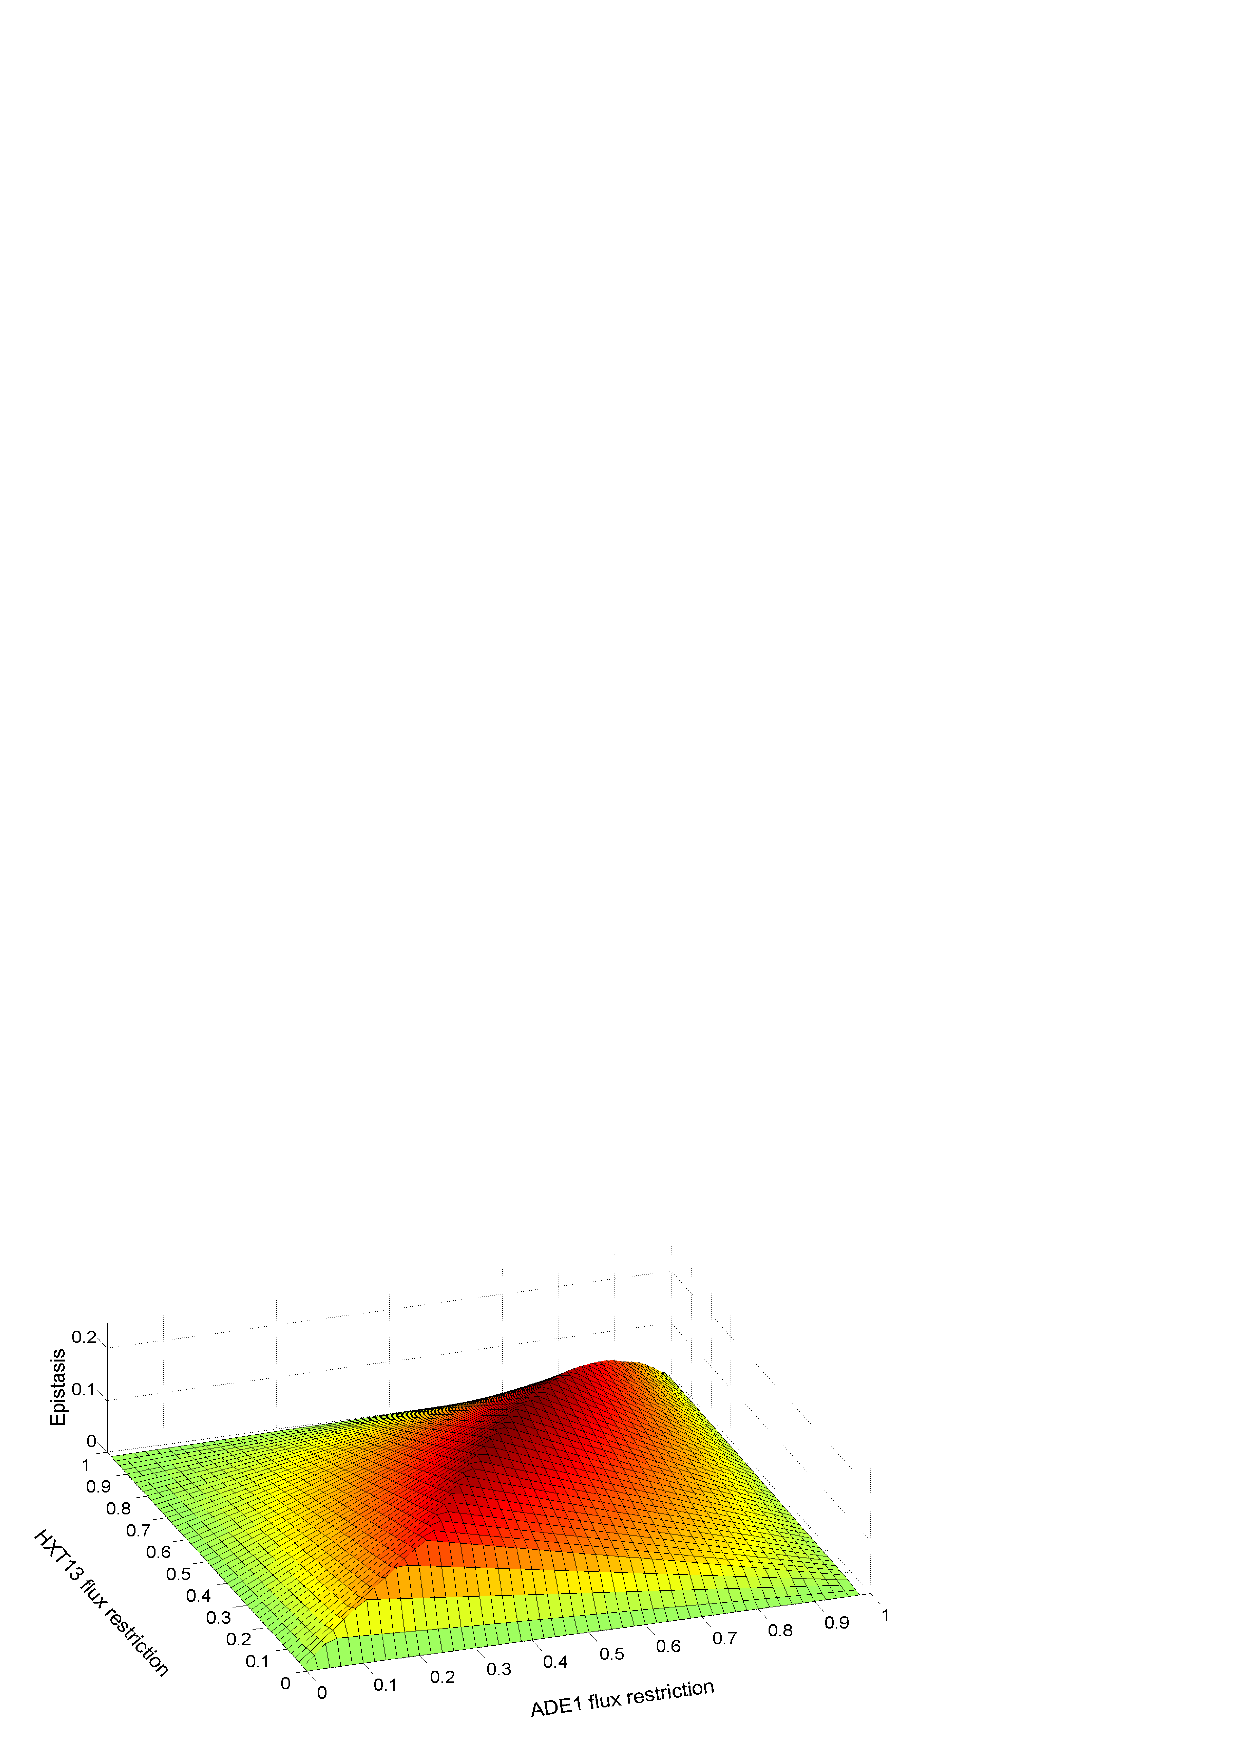
\includegraphics[width=\textwidth]{sgeFigure_S6}
\caption{An epistatic landscape exhibits smooth change in epistasis as
a function of the flux restriction for the genes HXT13 and ADE1. The
color corresponds to the z-axis (epistasis), with red being more
positive, and green being near zero. See dataset S3 for simulated
data. HXT13 is a hexose transporter and ADE1 is required for de novo
purine biosynthesis. The epistasis surface for HXT13 and ADE1 is quite
smooth, which is a fairly common pattern and we may infer that
epistasis, at least in metabolism, is often dependant on thresholds.}
\label{fig:sgeS6}
\end{figure}

\begin{figure}[H]
\centering
  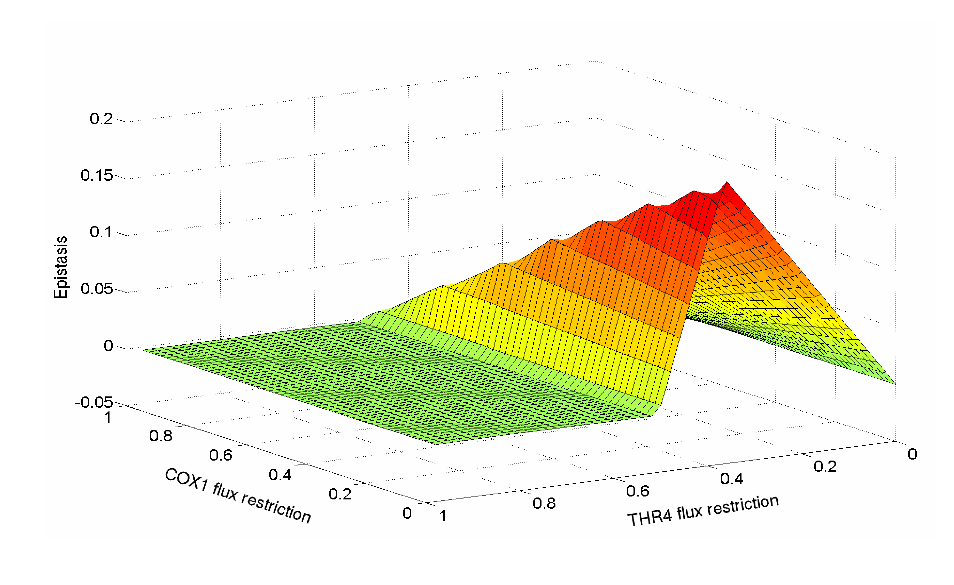
\includegraphics[width=\textwidth]{sgeFigure_S7}
\caption{An epistatic landscape exhibits a sharp transition to zero
epistasis, primarily as a consequence of the THR4 flux
restriction. The color corresponds to the z-axis (epistasis), with red
being more positive, and green being near zero. See dataset S4 for
simulated data. Epistasis is examined between threonine synthase gene
THR4 and COX1 (subunit 1 of cytochrome c oxidase). Both genes are
associated with mutually exclusive reactions. As shown in the figure,
there are regions where the epistasis is effectively zero (on the
order of 10-5) where the THR4 single mutant growth rate has only
changed very slightly, effectively allowing the mutations to act
independently. Once the THR4 mutant becomes more severe, the effects
are no longer independent.}
\label{fig:sgeS7}
\end{figure}

\begin{figure}[H]
\centering
  \includegraphics[width=\textwidth]{sgeFigure_S8}
\caption{A flow chart to illustrate the simulation process that
generates Fig. 4B. This procedure included 5 steps as indicated in the
5 blue boxes, and we have repeated step 2 to step 5 in the simulation
to produce all possible allele combinations, as highlighted in the red
box.}
\label{fig:sgeS8}
\end{figure}

\section{Supporting Data}

Supporting datasets S1-S4 are available online (\texttt{DOI:
10.1073/pnas.1121507109}).